% RUNNING MAN
%% https://tex.stackexchange.com/questions/441917/is-there-a-simple-way-to-use-stick-figures-into-pgf-tikz-drawings


\documentclass{standalone}


% DELTA FUNCTION - GAUSSIAN FUNCTION
%% https://www.researchgate.net/publication/258379289_Stability_and_Numerical_Analysis_of_the_Hebraud-Lequeux_Model_for_Suspensions?_tp=eyJjb250ZXh0Ijp7ImZpcnN0UGFnZSI6Il9kaXJlY3QiLCJwYWdlIjoicHVibGljYXRpb25Eb3dubG9hZCIsInByZXZpb3VzUGFnZSI6Il9kaXJlY3QifX0
%% DOI: 10.1155/2011/415921
%% https://tikz.net/delta_function/

% GAUSSIAN WAVE PACKET
%% https://tikz.net/delta_function/

% RUNNING MAN
%% https://tex.stackexchange.com/questions/441917/is-there-a-simple-way-to-use-stick-figures-into-pgf-tikz-drawings




\IfStandalone{\def\datapath{../../../}}{\def\datapath{}}

\input{\datapath QT-Notes-Preambles/QT-Notes-Diagrams-and-Graphs-DEFAULT-Preamble.tex}



% https://tex.stackexchange.com/questions/441917/is-there-a-simple-way-to-use-stick-figures-into-pgf-tikz-drawings
\usepackage{tikzsymbols}
%\usetikzlibrary{shapes.symbols}


\begin{document}
	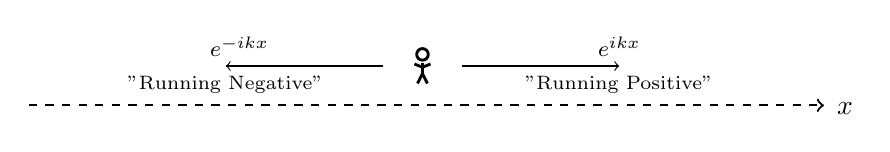
\begin{tikzpicture}
		\def\xmin{-5} % min x axis
		\def\xmax{5}     % max x axis
		
		\draw[->,thick,dashed] (-\xmax,0) -- (\xmax+0.1,0) node[below=1,right=1] {$x$};
		
		\node at (0,0.5) {\Strichmaxerl[2]};
		\draw[->] (-0.5,0.5) -- ({0.5*\xmin},0.5) node[left=-5,above] {\footnotesize $e^{-ikx}$} node[below] {\scriptsize ''Running Negative''};
		\draw[->] (0.5,0.5) -- ({0.5*\xmax},0.5) node[right,above] {\footnotesize $e^{ikx}$} node[below] {\scriptsize ''Running Positive''};
		
	\end{tikzpicture}
\end{document}